\begin{minipage}{\textwidth}
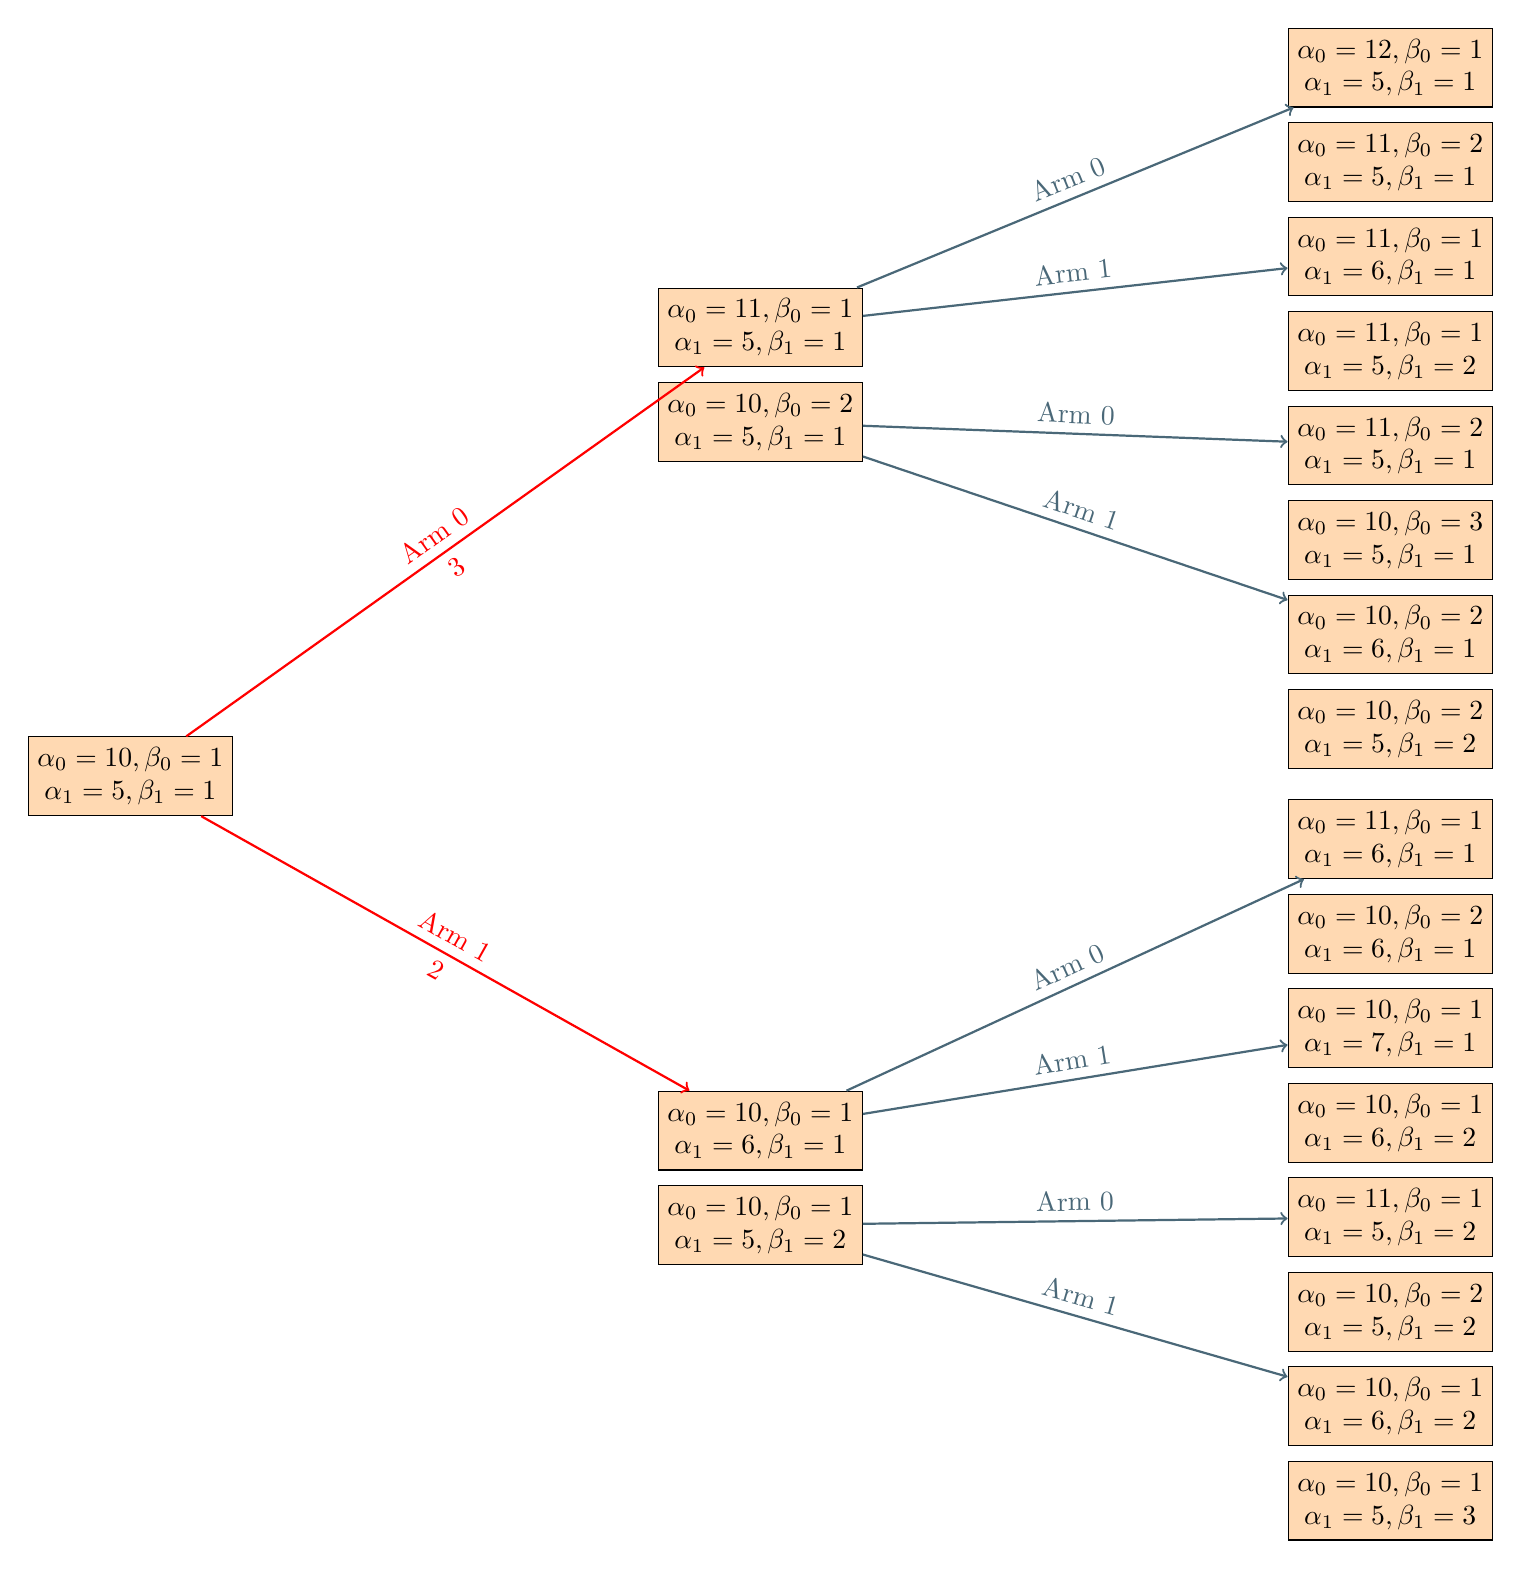
\begin{tikzpicture}
\tikzstyle{state} = [rectangle, text centered, minimum width=1.2cm, minimum height=1cm, draw=black, fill=orange!30]
\node[state] at (-10,0)  (h0){\shortstack{$\alpha_0=10, \beta_0=1$ \\ $\alpha_1=5, \beta_1=1$}};
\node[state] at (-2, 5.7) (h1_0){\shortstack{$\alpha_0=11, \beta_0=1$ \\ $\alpha_1=5, \beta_1=1$}};
\node[state] at (-2, 4.5) (h1_1){\shortstack{$\alpha_0=10, \beta_0=2$ \\ $\alpha_1=5, \beta_1=1$}};
\node[state] at (-2, -4.5) (h1_2){\shortstack{$\alpha_0=10, \beta_0=1$ \\ $\alpha_1=6, \beta_1=1$}};
\node[state] at (-2, -5.7) (h1_3){\shortstack{$\alpha_0=10, \beta_0=1$ \\ $\alpha_1=5, \beta_1=2$}};
\node[state] at (6, 9) (h2_0){\shortstack{$\alpha_0=12, \beta_0=1$ \\ $\alpha_1=5, \beta_1=1$}};
\node[state] at (6, 7.8) (h2_1){\shortstack{$\alpha_0=11, \beta_0=2$ \\ $\alpha_1=5, \beta_1=1$}};
\node[state] at (6, 6.6) (h2_2){\shortstack{$\alpha_0=11, \beta_0=1$ \\ $\alpha_1=6, \beta_1=1$}};
\node[state] at (6, 5.4) (h2_3){\shortstack{$\alpha_0=11, \beta_0=1$ \\ $\alpha_1=5, \beta_1=2$}};
\node[state] at (6, 4.2) (h2_4){\shortstack{$\alpha_0=11, \beta_0=2$ \\ $\alpha_1=5, \beta_1=1$}};
\node[state] at (6, 3.0) (h2_5){\shortstack{$\alpha_0=10, \beta_0=3$ \\ $\alpha_1=5, \beta_1=1$}};
\node[state] at (6, 1.8) (h2_6){\shortstack{$\alpha_0=10, \beta_0=2$ \\ $\alpha_1=6, \beta_1=1$}};
\node[state] at (6, 0.6) (h2_7){\shortstack{$\alpha_0=10, \beta_0=2$ \\ $\alpha_1=5, \beta_1=2$}};
\node[state] at (6, -0.8) (h2_8){\shortstack{$\alpha_0=11, \beta_0=1$ \\ $\alpha_1=6, \beta_1=1$}};
\node[state] at (6, -2) (h2_9){\shortstack{$\alpha_0=10, \beta_0=2$ \\ $\alpha_1=6, \beta_1=1$}};
\node[state] at (6, -3.2) (h2_10){\shortstack{$\alpha_0=10, \beta_0=1$ \\ $\alpha_1=7, \beta_1=1$}};
\node[state] at (6, -4.4) (h2_11){\shortstack{$\alpha_0=10, \beta_0=1$ \\ $\alpha_1=6, \beta_1=2$}};
\node[state] at (6, -5.6) (h2_12){\shortstack{$\alpha_0=11, \beta_0=1$ \\ $\alpha_1=5, \beta_1=2$}};
\node[state] at (6, -6.8) (h2_13){\shortstack{$\alpha_0=10, \beta_0=2$ \\ $\alpha_1=5, \beta_1=2$}};
\node[state] at (6, -8) (h2_14){\shortstack{$\alpha_0=10, \beta_0=1$ \\ $\alpha_1=6, \beta_1=2$}};
\node[state] at (6, -9.2) (h2_15){\shortstack{$\alpha_0=10, \beta_0=1$ \\ $\alpha_1=5, \beta_1=3$}};
\begin{scope}[cyan!40!black]
\draw[thick, ->, red] (h0) -- (h1_0) node[sloped, pos=0.5, above] {Arm $0$} node[sloped, pos=0.5, below]{3};
\draw[thick,->, red] (h0) -- (h1_2) node[sloped, pos=0.5, above] {Arm $1$} node[sloped, pos=0.5, below]{2};
\draw[thick,->] (h1_0) -- (h2_0) node[sloped, pos=0.5, above] {Arm $0$};
\draw[thick,->] (h1_0) -- (h2_2) node[sloped, pos=0.5, above] {Arm $1$};
\draw[thick,->] (h1_1) -- (h2_4) node[sloped, pos=0.5, above] {Arm $0$};
\draw[thick,->] (h1_1) -- (h2_6) node[sloped, pos=0.5, above] {Arm $1$};
\draw[thick,->] (h1_2) -- (h2_8) node[sloped, pos=0.5, above] {Arm $0$};
\draw[thick,->] (h1_2) -- (h2_10) node[sloped, pos=0.5, above] {Arm $1$};
\draw[thick,->] (h1_3) -- (h2_12) node[sloped, pos=0.5, above] {Arm $0$};
\draw[thick,->] (h1_3) -- (h2_14) node[sloped, pos=0.5, above] {Arm $1$};
\end{scope}
\end{tikzpicture}
\end{minipage}
